\mainmatter%
\setcounter{page}{1}

\lectureseries[\course]{\course}

\auth[\lecAuth]{Lecturer: \lecAuth\\ Scribe: \scribe}
\date{October 15, 2009}

\setaddress%

% the following hack starts the lecture numbering at 6
\setcounter{lecture}{5}
\setcounter{chapter}{5}

\lecture{Inventory Control and Infinite Time Horizon}

\section{Inventory Control}
This is a continuation of Lecture 5 and looking at the inventory control problem\footnote{Additional material for this section can be found in the class handout, specifically ``The Dynamic Programming Algorithm'' by Dimitri Bertsekas from the book
\href{http://www.amazon.com/Dynamic-Programming-Deterministic-Stochastic-Models/dp/0132215810}{``Dynamic Programming: Deterministic and Stochastic Models''}.}.
The system is given by
\begin{align*}
\xi_{t+1} = \xi_t+u_t+w_t, \qquad u_t\in\mathcal{U} = [0,\infty), \\% chktex 9
\{w_t\} = \text{IID}, \qquad w_t(\w) \in (-\infty,0]~\forall \w\in\Omega% chktex 9
\end{align*}
The cost is given by
\begin{align*}
J(s,x,\mu) &= E\left\lbrace\sum_{t=s}^{T-1} cu_t + p\max\{0,-(\xi_t+u_t+w_t)\} \right. \\
&\left. \qquad + h\max\{0,\xi_t+u_t+w_t\}\right\rbrace
\end{align*}
with $\phi=0$.
Note that $V(T,x)=0$ indicating zero terminal cost, $\xi_{t+1}<0$ implying ``backlogged'' inventory, $u_t=\mu_t(\xi_k)$, $y=x+u$, $u\geq 0\Leftrightarrow y\geq x$.
We will assume that $V(t+1,\cdot)$ is convex, with $\cdot$ representing the state of the system.
Also, let $\bar{y}\in\arg\min H_t(y)$.
We will also propose that if $H$ is convex on $\mathbb{R}$ and $\bar{y}\in\arg\min H_t(y)$ then $H_t$ is monotonically increasing on $[\bar{y},\infty)$ and monotonically decreasing on $(-\infty,\bar{y}]$.% chktex 9

Using this information the value function is given by
\begin{align*}
V(t,x) &= \inf_{u\geq 0} \{c(u+x) + pE_w[\max(0,-(\xi_t+u_t+w_t))] \\
&+ hE_u[\max(0,\xi_t+u_t+w_t)] + E_w[V(t+1,x+u+w)]\} - cx \\
&= \inf_{u\geq 0} \{H_t(x+u)\} - cx \\
&= \inf_{y\geq x}\{H_t(y)\} - cx \\
&= \begin{cases} H_t(\bar{y})-cx, & x\leq\bar{y} \\ H_t(x)-cx, & x>\bar{y} \end{cases}
\end{align*}
Notice that each term in $V(t,x)\geq 0 \Rightarrow V(t,x)\geq 0$.
Also, $V(t+1,x)\geq 0~\forall x \Rightarrow H_t(y)\to\infty \text{~as~} |y|\to\infty \therefore \exists \min$.

Using this value function gives
$$y^{\text{opt}} = \begin{cases} \bar{y}, & x\leq\bar{y} \\ x & x\geq y \end{cases}$$
and leads to an optimal control policy of
$$\mu_t = y^{\text{opt}}-x = \begin{cases} \bar{y}-x, & x\leq\bar{y} \\ 0, & x>\bar{y} \end{cases}$$
We used that $V(t+1,\cdot)$ is convex  so to induction we still need to show that $V(t,\cdot)$ is convex to complete the proof.

\begin{theorem}
$V(t,\cdot)$ is convex.
\end{theorem}

\begin{proof}
It is sufficient to show that
$$U_t(x) = \begin{cases} H_t(\bar{y}), & x\leq\bar{y} \\ H_t(x), & x>\bar{y} \end{cases}$$
is convex.
There are three cases that must be considered, see Figure~\ref{fig:06curve}.
Let $x_1,x_2\in\mathbb{R}$, $\lambda\in[0,1]$, $z_\lambda = \lambda x_1 + (1-\lambda)x_2$.
Then
\begin{enumerate}
\item $x_1,x_2\geq\bar{y} \Rightarrow U_t(x) = H_t(x)$
\item $x_1,x_2\leq\bar{y} \Rightarrow U_t(x_1) = U_t(x_2) = U_t(z_\lambda) = H_t(\bar{y})$
\item $x_1\leq\bar{y}\leq z_\lambda\leq x_2$
\end{enumerate}
(c) can be proved by noting that $H_t$ is convex and monotonically increasing to the right of $\bar{y}$ and using $\beta\geq\lambda$ as a constant.
\begin{align*}
z_\lambda &= \beta\bar{y} + (1-\beta)x_2 \\
H_t(z_\lambda) &\leq \beta H_t(\bar{y})+(1-\beta)H_t(x_2) \\
&= \lambda H_t(\bar{y})+(\beta-\lambda)H_t(\bar{y}) + (1-\lambda)H_t(x_2) + (\lambda-\beta)H_t(x_2) \\
&\leq \lambda H_t(\bar{y}) + (1-\lambda)H_t(x_2) \\
&= \lambda U_t(x_1) + (1-\lambda)U_t(x_2)
\end{align*}
\end{proof}

\begin{figure}[ht!]
\centering
\includegraphics[width=.5\textwidth]{images/06curve}
\caption{Convex curve.}
\label{fig:06curve}
\end{figure}

\section{Infinite Time Horizon, Discounted Cost}
The system is given as
\begin{align*}
\xi_{t+1} = f(\xi_t,u_t,w_t), \qquad \xi_0 = x
\end{align*}
The cost is
\begin{align*}
J(x,\mu) = E_{w_{]0,\infty[}}\left\lbrace\sum_{t=0}^\infty \alpha^t l(\xi_t,\mu_t(\xi_t))\right\rbrace, \qquad \alpha\in(0,1)% chktex 9
\end{align*}
Note that a smaller $\alpha$ implies more myopic behavior and $\alpha=0$ implies a completely greedy controller.
If
$$|l(x,u)|\leq L \Rightarrow J(x,\mu)\leq E\left\lbrace\sum_{t=0}^\infty \alpha^T L\right\rbrace \leq \frac{1}{1-\alpha}L<\infty$$

\begin{example}
Given $\xi_{t+1}=u_t\xi_t$, $\mu_t(\xi_t)=2$, $\xi_t=2^t x$ and $\alpha=3/4$ gives
  $$J(x,\mu) = \sum{\left(\frac{3}{4}\right)}^t 2^t x\to+\infty$$
$\lozenge$
\end{example}

An alternative method for solving this type of problem is to average the cost per unit time such that
$$J(x,\mu) = \lim_{T\to\infty}\sup \frac{1}{T}E\left[\sum_{t=0}^T l(xi_t,u_t)\right]$$
This is used in non-linear $H_\infty$.
We are not going to spend time on this method in this course though.

\subsection{Dynamic Programming Principle}
$$V(x) = \inf_{\mu\in\mathcal{M}_{0,\infty}} J(x,\mu)$$
The following is \textit{not} a proof and we are assuming Markov processes.
Let $r=t-\tau$, $\hat{\xi}_r=\xi_{\tau+r}$, $\hat{\mu}_r=\mu_{\tau+r}$ and $\hat{w}_r=w_{\tau+r}$.
Then we can get the value function as
\begin{align}
V(x) &= \inf_{\mu\in\mathcal{M}_{0,\infty}} E_{w_{]0,\infty[}} \left\lbrace \sum_{t=1}^{T-1} \alpha^t l(\xi_t,\mu_t(\xi_t)) + \sum_{t=-\tau}^\infty \alpha^t l(\xi_t,\mu_t(\xi_t))\right\rbrace \nonumber \\% chktex 9
&= \inf_{\mu\in\mathcal{M}_{0,\infty}} E_{w_{]0,\infty[}} \left\lbrace \sum_{t=1}^{T-1} \alpha^t l(\xi_t,\mu_t(\xi_t)) \right. \nonumber \\% chktex 9
&\left. \qquad +  \alpha^t \sum_{r=0}^\infty \alpha^r l(\xi_{\tau+r},\mu_{\tau+r}(\xi_{\tau+r})) \right\rbrace \nonumber \\
&= \inf_{\mu\in\mathcal{M}_{\mu_{]0,\tau-1[}}} E_{]0,\tau-1[} \left\lbrace \sum_{t=0}^{\tau-1} \alpha^t l(\xi_t,\mu_t(\xi_t))\right\rbrace \nonumber \\% chktex 9
&\qquad + \alpha^\tau\inf_{\mu\in\mathcal{M}_{\mu_{]\tau,\infty[}}} E_{w_{]\tau,\infty[}} \left\lbrace \sum_{r=0}^\infty\alpha^r l(\xi_{\tau+r},\mu_{\tau+r}(\xi_{\tau+r}))\right\rbrace \nonumber \\% chktex 9
&= \inf_{\mu\in\mathcal{M}_{]0,\tau-1[}} E_{\mu_{]0,\tau-1[}} \left\lbrace \sum_{t=0}^{\tau-1} l(\xi_t,\mu(\xi_t)) \right. \nonumber \\% chktex 9
&\left. \qquad + \alpha^\tau \inf_{\mu\in\mathcal{M}_{]0,\tau-1[}} \sum_{r=0}^\infty \alpha^r l(\hat{\xi}_r,\hat{\mu}_r(\hat{\xi}_r)) \right\rbrace \nonumber \\% chktex 9
&= \inf_{\mu\in\mathcal{M}_{]0,\tau-1[}} E_{\mu_{]0,\tau-1[}} \left\lbrace \sum_{t=0}^{\tau-1} l(\xi_t,\mu(\xi_t)) + \alpha^\tau V(\xi_\tau) \right\rbrace \nonumber \nonumber \\% chktex 9
\Rightarrow V(x) &= \inf_{\mu\in\mathcal{M}_{]0,\tau-1[}} E_{\mu_{]0,\tau-1[}} \left\lbrace \sum_{t=0}^{\tau-1} l(\xi_t,\mu(\xi_t)) + \alpha^\tau V(\xi_\tau) \right\rbrace% chktex 9
\end{align}
This is the dynamic programming principle (DPP)! When $\tau=1$ we get the Dynamic Programming Equation (DPE).

\subsection{Dynamic Programming Equation}
\begin{align}
V(x) &= \inf_{\mu\in\mathcal{M}_{0,0}} E_{\mu_0} \left\lbrace l(x,\mu_0(x)) + \alpha V(\xi_1) \right\rbrace \nonumber \\
\Rightarrow V(x) &= \inf_{u\in\mathcal{U}} \left\lbrace l(x,u) + \alpha E_w[V(f(x,u,w))] \right\rbrace
\end{align}
This is the Dynamic Programming Equation! To get the minimum we have to solve for $V$, the value function.
If $\min\exists$ then
$$\mu(x)\in\arg\min\{l(x,u)+\alpha E_u[V(f(x,u,w))]\}$$
The DPE is of the form $V=\mathcal{G}[V]$, where $\mathcal{G}$ is a non-linear operator that maps one function to another function.
It is a recursive operator.
$$\mathcal{G}[\vp](x) = \inf_u\{l(x,u)+\alpha E_u[\vp(f(x,u,w))]\}$$

There are two methods that can be used to solve the DPE\@: value iteration (contraction mapping principle) and policy iteration.

\section{Normed Vector Space Review}
\label{sec:normedvectorspace}
\begin{definition}
A space is a set.
\end{definition}

\begin{definition}
$\mathcal{X}$ is a real vector space if $\alpha x+\beta y\in\mathcal{X}~\forall x,y\in\mathcal{X},~\forall \alpha\beta\in\mathbb{R}$.
\end{definition}

\begin{definition}
Let $\vectornorm{\cdot}: \mathcal{X}\to[0,\infty)$, not including $+\infty$, then $(\mathcal{X},\vectornorm{\cdot})$ is a normed vector space if% chktex 9
\begin{enumerate}
\item $\vectornorm{y}\geq0~\forall y\in\mathcal{X}$ and $\vectornorm{y}=0\Leftrightarrow y=0$
\item $||cy|| = |c|\vectornorm{y}~\forall c\in\mathbb{R}, y\in\mathcal{X}$
\item $\vectornorm{x+y}\leq ||x|| + ||y||$, $x,y\in\mathcal{X}$
\end{enumerate}
\end{definition}

\begin{example}
$\mathbb{R}^2$, $||x||=\sqrt{x_1^2+x_2^2}$
$\lozenge$
\end{example}

\begin{example}
$\mathcal{X}=\mathbb{R}^2$ with $||x|| = \max\{|x_1|,|x_2|\}$
$\lozenge$
\end{example}

\begin{example}
$\mathcal{X} = \mathbb{R}^2$, $||x||=|x_1|+|x_2|$
$\lozenge$
\end{example}

\begin{example}
$\mathcal{X} = C([a,b]) = \{y:[a,b]\to\mathbb{R} | \text{~continuous}\}$ and $||y|| = \max\{|y(t)| | t\in[a,b]\}$.
Do the conditions hold?
\newline
(a) $||y|| = \max\{|y(t)| | t\in[a,b]\}\geq 0$ holds and if $||y||=0 \Rightarrow \max\{|y(t)|\} = 0 \Rightarrow y(t)=0~\forall t$ holds.
\newline
(c) $||x+y|| = \max_{t\in[a,b]}\{|x(t)+y(t)|\} \leq \max_t\{|x(t)|+|y(t)|\} \leq \max_t\{|x(t)|\} + \max_t\{|y(t)|\} = ||x|| + ||y||$ holds.
$\lozenge$
\end{example}

\begin{example}
Let $B_R=B_R(0)\subset\mathbb{R}^n$ is
\begin{align*}
B_R(0) &= \{x\in\mathbb{R}^n | ||x||\subset R\} \\
\overline{B_R(0)} &= \overline{B_R} = \{x\in\mathbb{R}^n | ||x||\leq R\}
\end{align*}
and let $\mathcal{X}=C(\overline{B_R(0)}$.
Then
$$||y||=\max_{x\in B_R} |y(x)|$$
$\lozenge$
\end{example}% chktex 17
